\section{Discussion}

\subsection{Spatiality and Networks}
When trying to emulate the dynamics of the SIR model using an agent-based approach the question arises what we ultimately gain from doing so when we could have generated the dynamics much quicker and smoother using the system-approach. The difference is that the agent-based approach is a stochastic one and can thus also generate "degenerated" dynamics e.g. in which the disease dies out after a few steps or even can't spread from patient zero - in this case ABS is clearly a benefit as it allows to investigate \textit{alternative futures}, something not possible with system-dynamics in which the disease will never die out prematurely. 
The real benefits of ABS over the system-dynamics approach is that agents can be heterogeneous and make use of spatial- and/or network-information defining the neighbourhood. We can thus simulate the spread of the disease throughout a population which is laid out on e.g. a 2d-grid with holes in it or one can investigate spreading of the disease throughout a network of agents where some are vaccinated.
We provide already suitable environments to simulate these cases and show an example of spreading a disease on a 2d-grid in Figure \ref{fig:sir_spatial}.  

\begin{figure*}
\begin{center}
	\begin{tabular}{c c}
		\begin{subfigure}[b]{0.4\textwidth}
			\centering
			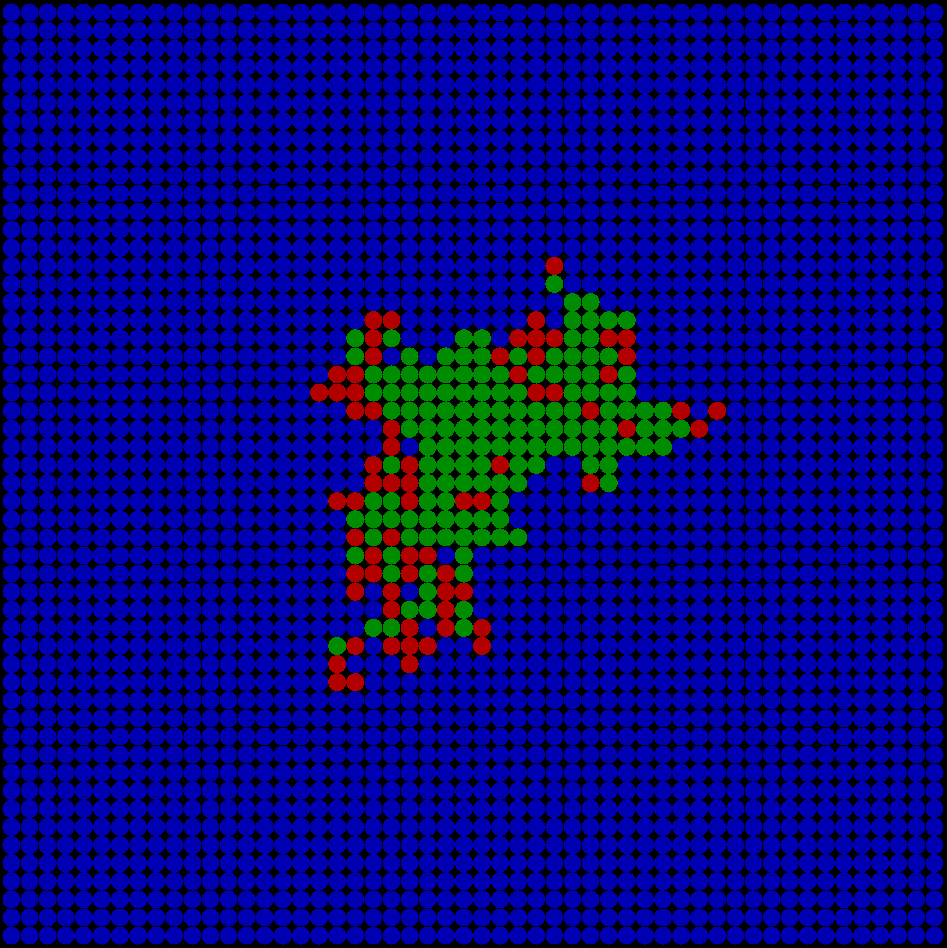
\includegraphics[width=.6\textwidth, angle=0]{./../shared/fig/SIR_spatial_52x52_92time.png}
			\caption{$t = 92$}
			\label{fig:sir_spatial_92}
		\end{subfigure}

		& 

		\begin{subfigure}[b]{0.4\textwidth}
			\centering
			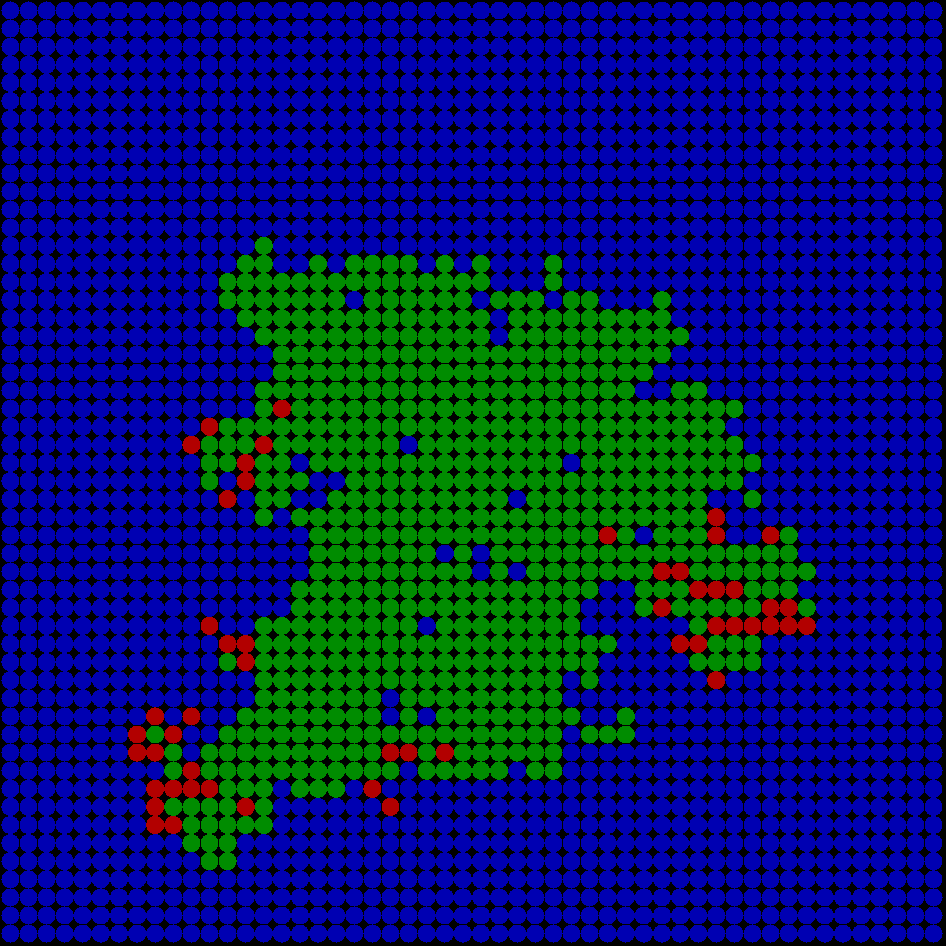
\includegraphics[width=.6\textwidth, angle=0]{./../shared/fig/SIR_spatial_52x52_200time.png}
			\caption{$t = 200$}
			\label{fig:sir_spatial_200}
		\end{subfigure}

		\\
		
		\begin{subfigure}[b]{0.4\textwidth}
			\centering
			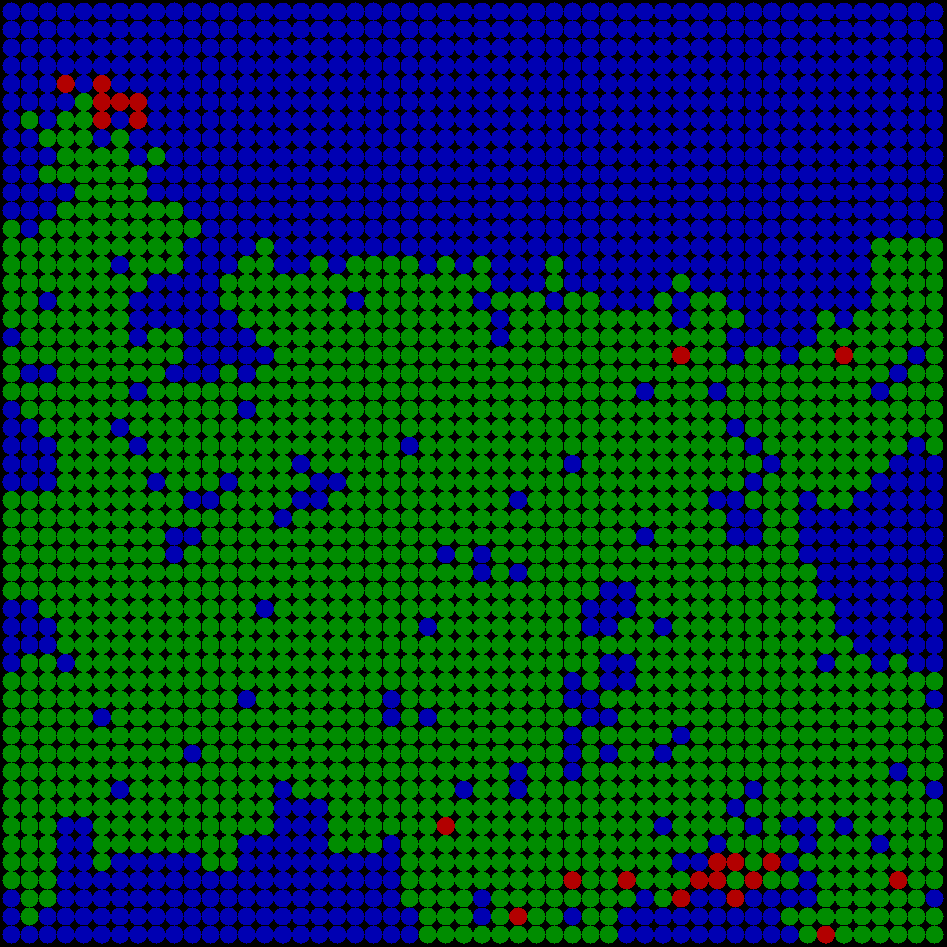
\includegraphics[width=.6\textwidth, angle=0]{./../shared/fig/SIR_spatial_52x52_440time.png}
			\caption{$t = 440$}
			\label{fig:sir_spatial_440}
		\end{subfigure}
		
		& 
		
		\begin{subfigure}[b]{0.4\textwidth}
			\centering
			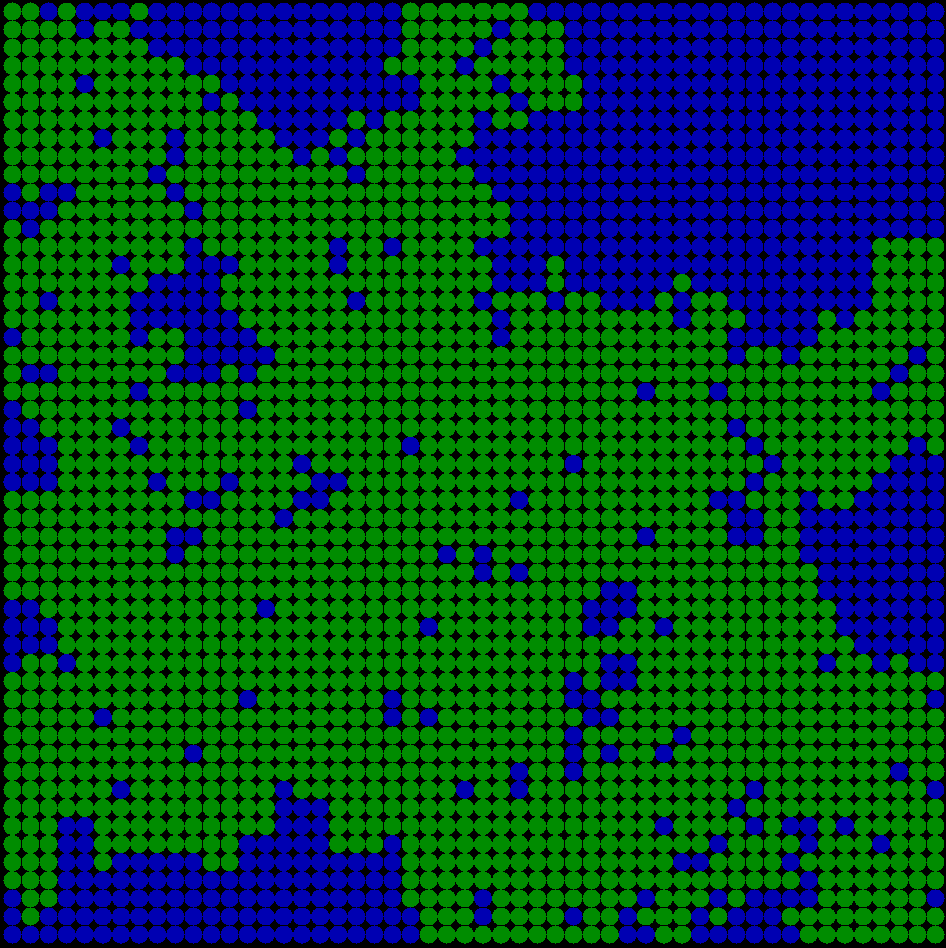
\includegraphics[width=.6\textwidth, angle=0]{./../shared/fig/SIR_spatial_52x52_873time.png}
			\caption{$t = 873$}
			\label{fig:sir_spatial_873}
		\end{subfigure}
	\end{tabular}
	
	\caption{Simulating SIR on a 52x52 grid with Moore neighbourhood. Blue are susceptible, red are infected, green are recovered. The green areas act as protection as infected cannot cross the recovered border: this is particularly visible in the lower right corner of \ref{fig:sir_spatial_440} where the disease has been contained in the blue island and has no means to escape. It may seem that the few remaining infected agents in the top left corner of \ref{fig:sir_spatial_440} will die out soon but still it needs more than the already running simulation-time until the disease actually dies out with the last patient recovering at center top of \ref{fig:sir_spatial_873} at $t = 873$.} 
	\label{fig:sir_spatial}
\end{center}
\end{figure*}

When using a 2d-grid or network one needs to setup them up in the initialization code so there is a little more work to do there but the implementation of the agents differ just in one single line, which is where the neighbourhood is picked TODO: refer to appendix code. Instead of \textit{randomAgentIdMsgSource} one uses either \textit{randomNeighbourNodeMsgSource} in the case of a network or \textit{randomNeighbourCellMsgSource} in case of a 2d-grid.

\subsection{Other Models}
TODO: mention that we have also implemented other models, which also work without time-semantics (all agents make a move at discrete time-steps and do not really rely on some notion of time). 

\subsection{Time-Semantics}
The main reason for building our pure functional ABMS approach on top of Yampa was to leverage the powerful time-semantics of Yampa which allows us to implement important concepts of ABMS:

state-chart: agents are at all time of their life-cycle in one state and can switch between multiple states using transitions 
timed transitions: transition to another state/behaviour happens at a discrete time
rate transitions: transition happens with a given rate
message transition: transition upon receiving a given message 

\subsection{Agents as Signals}
Due to the underlying nature and motivation of Functional Reactive Programming (und im speziellen) Yampa, Agents can be seen as Signals which is generated and consumed by a Signal-Function which is the behaviour of an Agent. If an Agent does not change the OUTPUT-signal is constant, if the agent changes e.g. by sending a message, changing its state,... the OUTPUT signal changes. A dead agent has no signal at all.

TODO: the FrSIR agents are true signals: they don't change when time does not change, this means they are completely time-dependent and only implemented using time-semantics. Agents of non-time semantic models like in the Schelling Segregation model won't exhibit this behaviour, they just act on every update and don't care about the time-delta and just assume that every update occurs after 1.0 dt.

TODO: the dynamics stay constant with a minor delay e.g. infected increases a bit while susceptible decreases. This is due to the delay of message delivery which takes one time-delta, independent of its value - messages are also delivered when time-delta is 0. Only message-generating functions which depend on non-zero dt to generate messages will then stop generate messages. Reactive functions which act on incoming messages can still create change as they do not rely on time-semantics but just on the discrete event of a message-arrival.


TODO: We implemented the function \textit{doRepeatedlyEvery} which transforms a non-time semantic agent-behaviour into one. It is built on Yampas \textit{repeatedly} function and has the following signature:


\subsection{Time-Sampling}
sampling rate depends on the transition times \& rates of the model. when e.g. the contact rate is 5 then the sampling dt should be below 0.2

\subsection{System Dynamics}
can emulate system dynamics due to the parallel update-strategy and continuous time-flow semantics

\subsection{Discrete Event Simulation}
DES in FrABMS? how easily can we implement server/queue systems? do they also look like a specification? potential problem: ordering of messages is not guaranteed by now

\subsection{Advantages}
advantages:
	- no side-effects within agents leads to much safer code
	- edsl for time-semantics
	- declarative style: agent-implementation looks like a model-specification
	- reasoning and verification
	- sequential and parallel
	- powerful time-semantics
	- arrowized programming is optional and only required when utilizing yampas time-semantics. if the model does not rely on time-semantics, it can use monadic-programming by building on the existing monadic functions in the EDSL which allow to run in the State-Monad which simplifies things very much
	- when to use yampas arrowized programing: time-semantics, simple state-chart agents 
	- when not using yampas facilities: in all the other cases e.g. SugarScape is such a case as it proceeds in unit time-steps and all agents act in every time-step
	- can implement System Dynamics building on Yampas facilities with total ease	
	- get replications for free without having to worry about side-effects and can even run them in parallel without headaches
	- cant mess around with time because delta-time is hidden from you (intentional design-decision by Yampa). this would be only very difficult and cumbersome to achieve in an object-oriented approach. TODO: experiment with it in Java - how could we actually implement this? I think it is impossible: may only achieve this through complicated application of patterns and inheritance but then has the problem of how to update the dt and more important how to deal with functions like integral which accumulates a value through closures and continuations. We could do this in OO by having a general base-class e.g. ContinuousTime which provides functions like updateDt and integrate, but we could only accumulate a single integral value.
	- reproducibility statically guaranteed
	- cannot mess around with dt
	- code == specification
	- rule out serious class of bugs
	- different time-sampling leads to different results e.g. in wildfire \& SIR but not in Prisoners Dilemma. why? probabilistic time-sampling?
	- reasoning about equivalence between SD and ABS implementation in the same framework
	- recursive implementations
	
	- we can statically guarantee the reproducibility of the simulation because: no side effects possible within the agents which would result in differences between same runs (e.g. file access, networking, threading), also timedeltas are fixed and do not depend on rendering performance or userinput	
	
\subsection{Disadvantages}
disadvantages:
	- performance is low
	- reasoning about performance is very difficult
	- very steep learning curve for non-functional programmers
	- learning a new EDSL
	- think ABMS different: when to use async messages, when to use sync conversations


[ ] important: increasing sampling freqzency and increasing number of steps so that the same number of simulation steps are executed should lead to same results. but it doesnt. why?
[ ] hypothesis: if time-semantics are involved then event ordering becomes relevant for emergent patterns. there are no tine semantics in heroes and cowards but in the prisoners dilemma
[ ] can we implement different types of agents interacting with each other in the same simulation ? with different behaviour funcs, digferent state? yes, also not possible in NetLogo to my knowledge. but they must have the same messages, emvironment 

[ ] Hypothesis: we can combine with FrABS agent-based simulation and system dynamics (this has been proved by example!)